\documentclass{beamer}

\title{1. DN pri predmetu Napredna računalniška orodja}
\author{Avtor: Tomaž Ulaga}
\date{\today}

\begin{document}

% 1. Prosojnica: Uvodna prosojnica z naslovom
\begin{frame}
    \titlepage
\end{frame}

% 2. Prosojnica: Kazalo vsebine
\begin{frame}{Kazalo}
    \tableofcontents
\end{frame}

% 3. Prosojnica: Vsebina datoteke naloga1_1.txt
\section{Vsebina datoteke naloga1\_1.txt}
\begin{frame}{Vsebina datoteke naloga1\_1.txt}
    \begin{itemize}
        \item Prva vrstica: naslov podatkov ("time [s]")
        \item Druga vrstica: število vrstic in podatkov v vsaki vrstici (100 vrstic podatkov, v vsaki vrstici po en)
        \item Preostale vrstice: podatki časa v sekundah
        \item MATLAB funkcija za uvoz podatkov
            \item Funkcija: \texttt{importdata()} \\
                \textbf{Vhodni podatki:} ime datoteke \\
                 \textbf{Izhod:} vektor časovnih vrednosti
    \end{itemize}
    
\end{frame}

% 4. Prosojnica: Graf P(t)
\section{Graf moči P(t)}
\begin{frame}{Graf moči P(t)}
    \begin{itemize}
        \item Prikazuje moč \( P \) v odvisnosti od časa \( t \)
    \end{itemize}
    \begin{figure}
        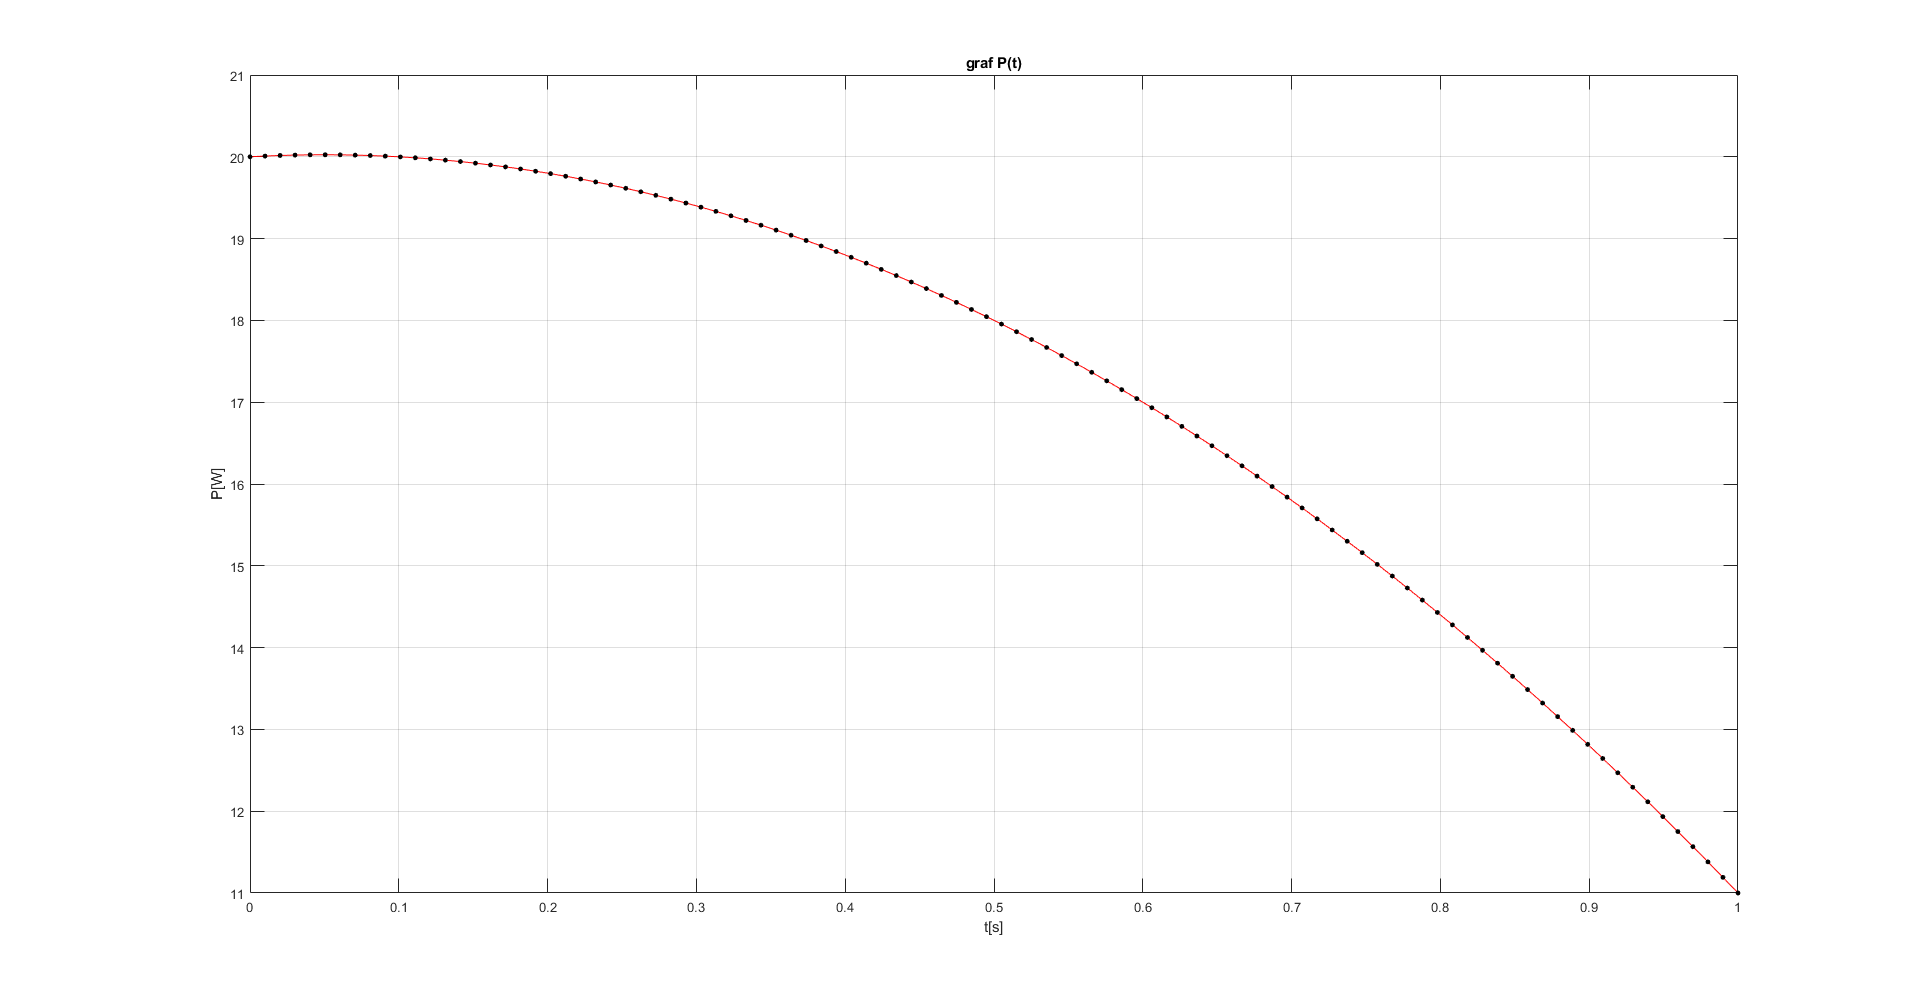
\includegraphics[width=1.1\textwidth]{graf_P_t_nro_dn1.png}
        \caption{Graf \( P(t) \)}
    \end{figure}
\end{frame}

% 5. Prosojnica: Trapezna formula in rezultat integracije
\section{Izračun integrala in trapezna metoda}
\begin{frame}{Izračun integrala in trapezna metoda}
    \begin{itemize}
        \item {Trapezna formula za integral}
        \[
        \int_{a}^{b} f(x) \, dx \approx \frac{\Delta x}{2} \left( f(x_0) + 2f(x_1) + 2f(x_2) + \dots + 2f(x_{n-1}) + f(x_n) \right)
        \]
        \item Rezultat integrala:izračunana vrednost integrala
        \( 
        \int_{t_{\text{min}}}^{t_{\text{max}}} P(t) \, dt \) je: \textbf{17,16650}
    \end{itemize}
\end{frame}

\end{document}
